%%%%%% 第3章 %%%%%%%%%%%%%%%%%%%%%%%%%%%
%
%\chapter{不良部品を考慮したFFSのマッチング処理制約} \label{sec:chapter3}
%
%\chaptermark{不良部品を考慮したFFSのマッチング処理制約}
%
%%ここから第2章からコピーしてきた文章
%
%\chaptermark{不良部品を考慮したFFSモデル}
%
%\section{不良部品が発生する場合のFFS\label{sec:furyo}}
%本論文では,前章で紹介した4工程FFSに対して各工程で不良部品が一定の確率で発生する状況を考慮する.
%具体的には,各工程で部品1個当たりの不良確率(不良部品が発生する確率)$\beta$を設ける.
%図$\ref{fig:queue2}$は不良部品の発生を考慮したFFSに対する待ち行列ネットワークを図示したものである.
%矢印の上についている$\beta$は,部品が矢印の先へ移動する確率を示している.
%
%%ここまで第2章からコピーしてきた文章

\chapter{Match processing constraint of FFS considering defective parts}

\chaptermark{Match processing constraint of FFS considering defective parts}

\chaptermark{FFS considering failure parts}

\section{FFS when failure parts occurs \label{sec:furyo}}
In this section, we consider the situation where failure parts occurs with a certain probability in each step of 4 step FFS introduced in the previous chapter.
Specifically, we set a failure probability (probability of occurence of a defective part) $\beta$ per part in each step.
Figure $\ref{fig;queue2}$ shows queuing network for a FFS in consideration of occurence of defective parts.
$\beta$ on the arrow indicates the probability of the parts moving to the buffer arrow is pointing.

\begin{figure}[ht]
	\begin{center}
		\includegraphics[clip, width=\hsize]{fig/queue-2.eps}
	\end{center}
	\caption{Queuing network model of FFS with removal or defective parts.}
	\label{fig:queue2}
\end{figure}


%\section{不良部品が発生する場合マッチング処理制約\label{sec:matching}}
%図$\ref{fig:ffs}$のFFSでは部品の順序が保持されるためマッチング処理制約が常に満たされていた.
%しかし,不良部品の廃棄を考慮した図$\ref{fig:queue2}$に対応するFFSでは,不良品の廃棄などにより部品の順序が保持されない.
%このような場合,第4工程でのマッチング処理制約を厳密に考慮する必要がある.
%そこで本章では,マッチング処理制約の影響を調べるため制約のある4工程FFSと制約のない4工程FFSの二つのFFSについて考える.
%マッチング処理制約のないFFSの場合,第2工程でのペアと関係なく,第4工程で二つの部品が揃ったときに組み合わせが開始できるものとした.
%図\ref{fig:FFSo}はマッチング処理制約のあるFFS,図\ref{fig:FFSx}はマッチング処理制約の無いFFSをGSPNで表したものである.
%本章では第1工程,第2工程,第4工程で発生した不良部品については即時に廃棄,マッチング処理制約の関係する第3工程で発生した不良部品に対しては第4工程で組み合わせる直前に廃棄するものとした.
%これはマッチング処理制約の無いFFSについても同様とする.
%\begin{figure}[p]
%\begin{center}
%	\includegraphics[height=\vsize]{FFSo.eps}
%\end{center}
%\caption{マッチング処理制約のある4工程FFSのGSPN}
%\label{fig:FFSo}
%\end{figure}

\section{Match processing constraint when defective part occur \label{sec:matching}}
In FFS shown by figure $\ref{fig:ffs}$, match processing constraint was always satisfied since the order of parts was always maintained.
However, in the FFS which considered the removal of defective parts, shown in figure $\ref{fig:queue2}$, the order of parts is not retained due to the discarding of defective parts. 
In this situation, we need to consider the match processing constraint in the fourth step strictly.
Therefore, in this chapter, we will consider two FFSs, 4 step FFS with and without constraint to investigate the influence of match processing constraint.
For FFS without constarint, we assume that regardless of the pair in the second step, conbination can be started when the two parts are gathered at fourth step.
Figure $\ref{fig:FFSo}$ shows the GSPN for FFS with constraint and figure $\ref{fig:FFSx}$ shows GSPN for FFS without constraint.
In this chapter, we assumed that defective parts generated in the first, second, and fourth step are immediately removed and defective parts generated in the third step, which is step related to match processing constraint, are removed before combination in the fourth step.
This assumption also applies to FFS without constraint.


\begin{figure}[p]
\begin{center}
	\includegraphics[height=\vsize]{fig/FFSo.eps}
\end{center}
\caption{GSPN for 4 step FFS with constraint.}
\label{fig:FFSo}
\end{figure}

\begin{figure}[p]
\begin{center}
	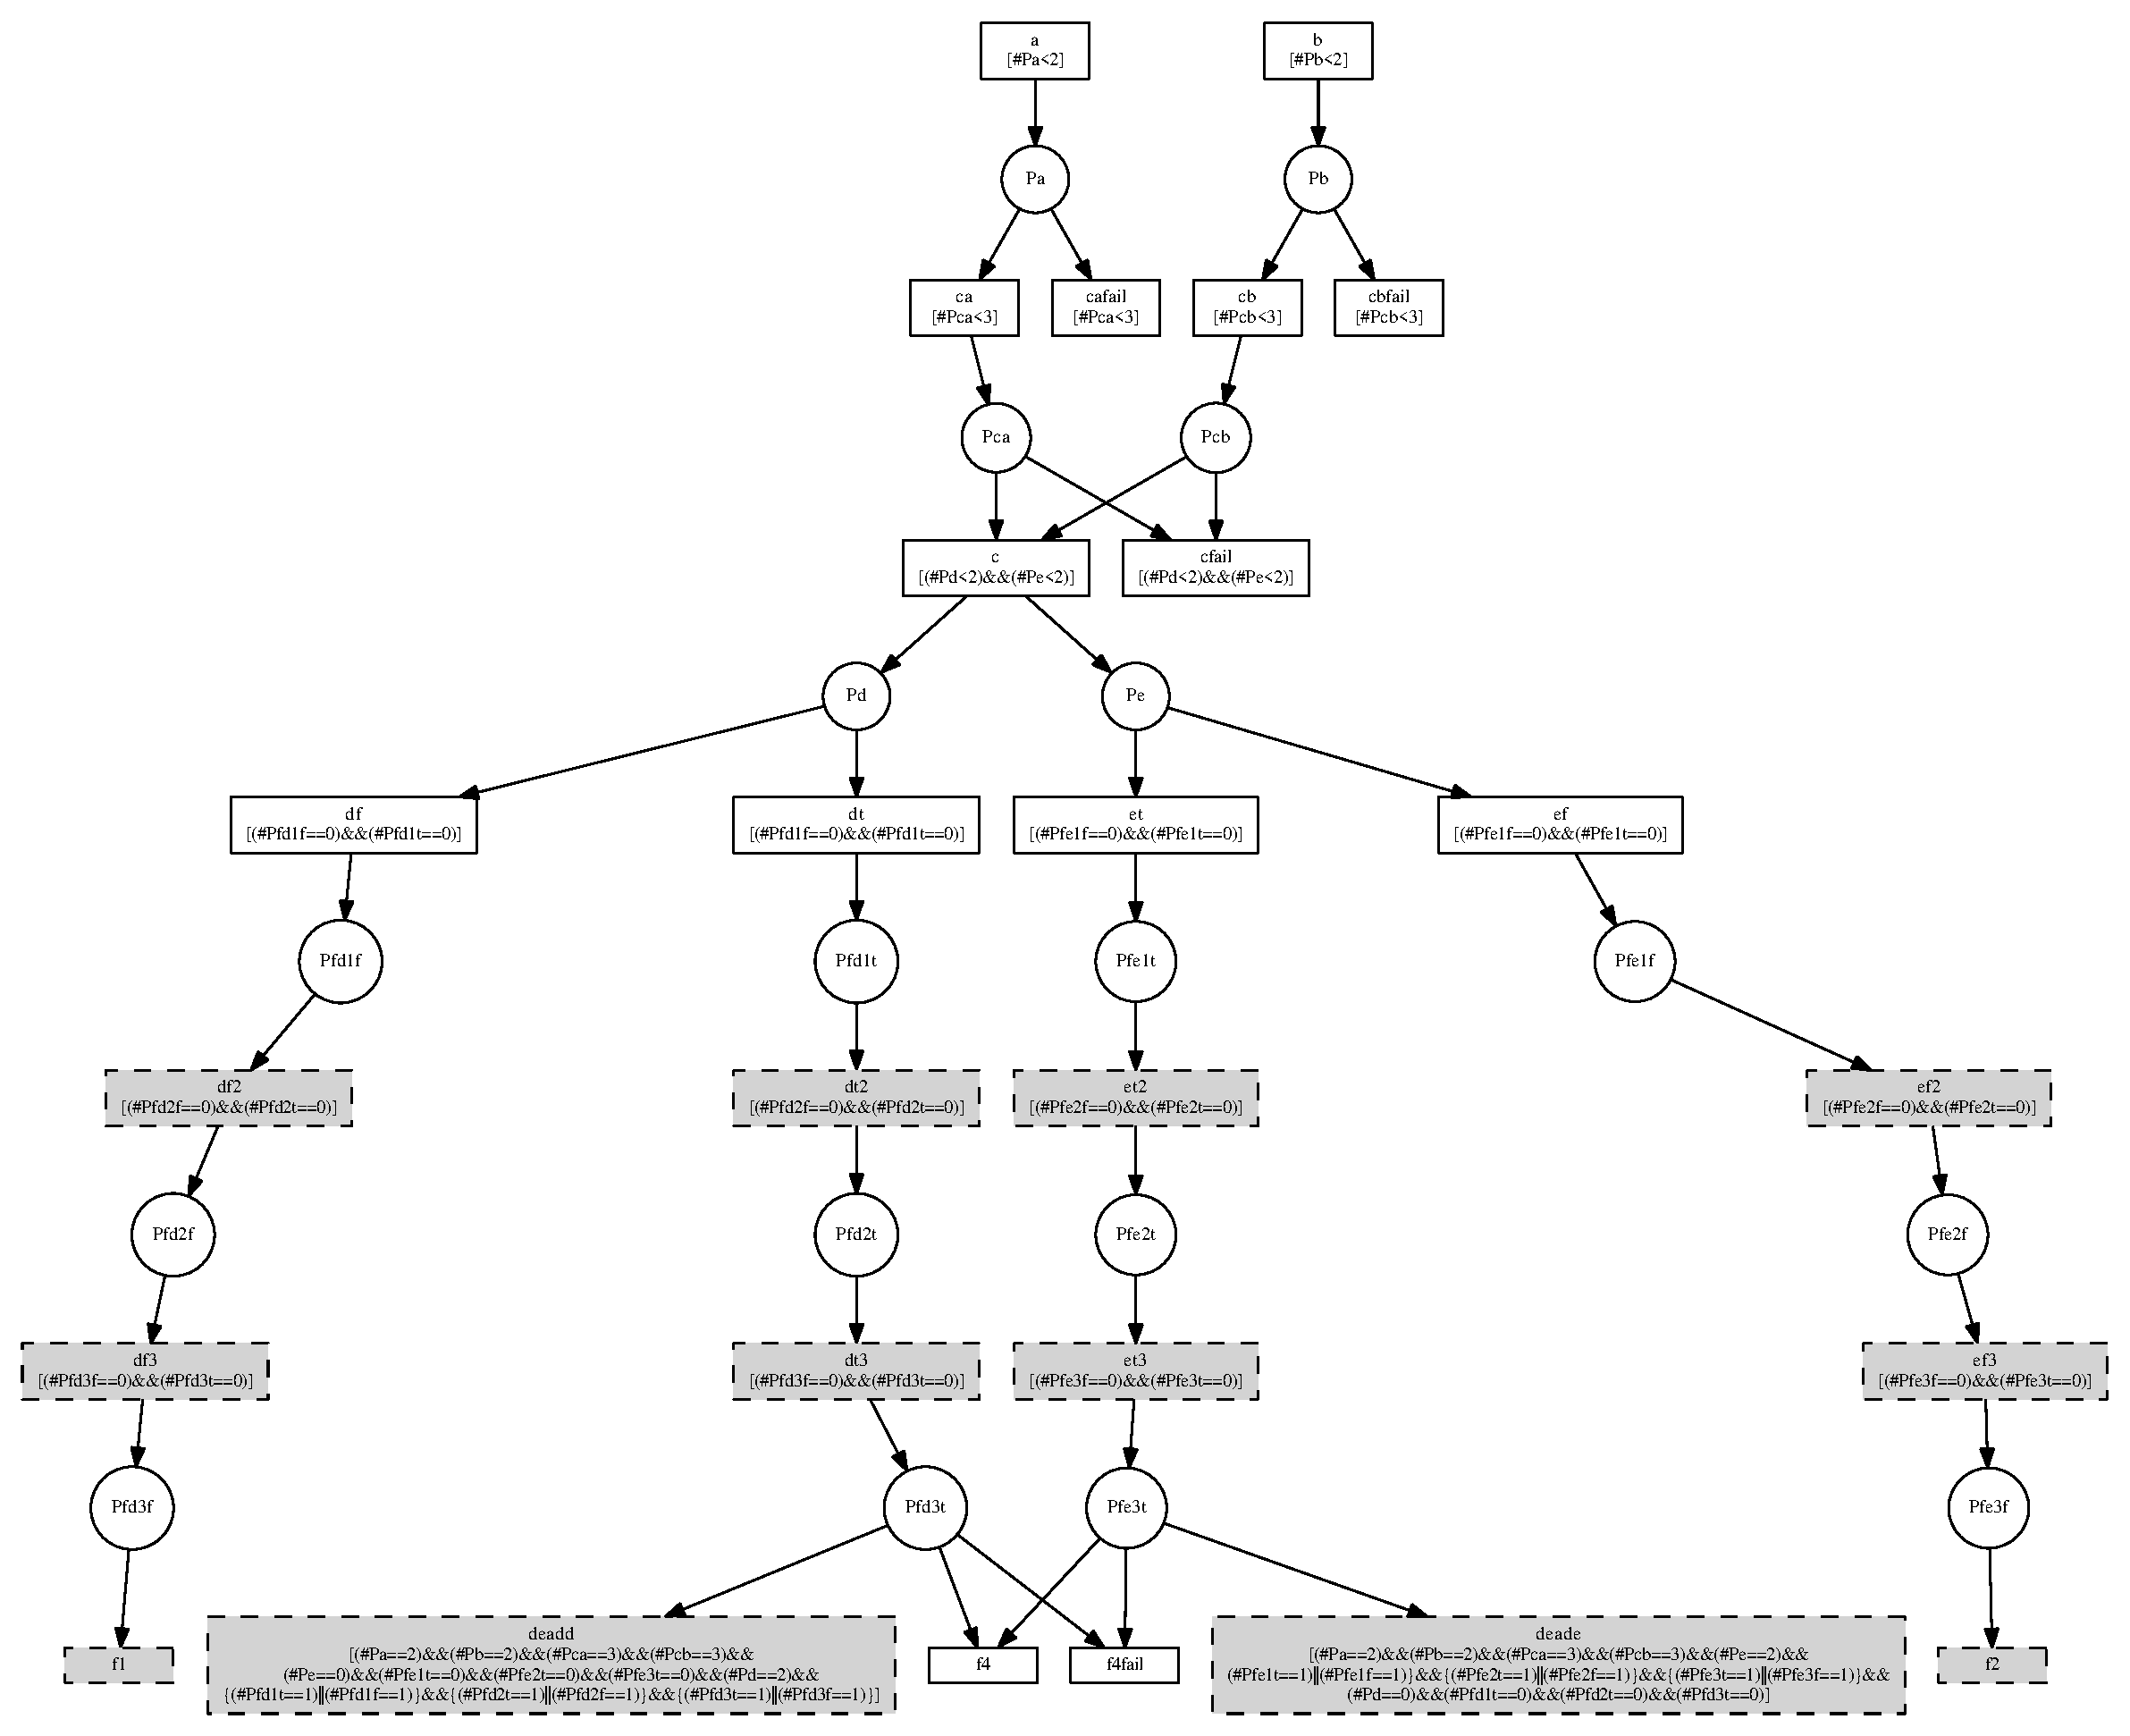
\includegraphics[width=\hsize]{fig/FFSx.eps}
\end{center}
\caption{GSPN for 4 step FFS without constraint.}
\label{fig:FFSx}
\end{figure}

\clearpage

%\section{数値実験}
%\ref{sec:matching}節で述べた二つFFSの待ち行列ネットワークモデルに対する性能評価を行う.
%性能指標としてスループットとブロッキング確率を算出する.
%スループットは単位時間あたりに第4工程で処理される部品数で定義する.
%また,ブロッキング確率は,定常状態において 第4工程のバッファに空きがない状態の確率を算出する.
%ここでは,二種類の部品に対して同じ到着率,処理率を仮定しているため,第3工程の一方のラインだけに注目し,そのブロッキング確率を算出している.
%また実験では,二つの別々のラインを持つ第1工程と第3工程のバッファの大きさを1(処理中の部品は含めない),組み合わせのある第2工程と第4工程における各部品のバッファの大きさをそれぞれ2とした.
%
%GSPN解析により,マッチング処理制約がない場合,第1工程と第2工程のすべてのバッファ及び,第3工程,第4工程のうちの片方のラインのバッファが全て埋まり,もう片方のバッファが全て空の状態で全行程の処理が停止する状況(デッドロック)が発生することが分かった.
%これを回避するため,マッチング処理制約がない場合ではデッドロック状態になると直ちに第4工程の正常な部品を廃棄し,システムが正常に稼働するようにした.
%
%処理率$\mu=1.0$の元で,二つの部品の到着率$\lambda$及び不良率$\beta$を変化させてスループット(TP)と第3工程におけるブロッキング確率(BP)を計算した結果が表\ref{tab:result09} から表 \ref{tab:result001}である.

\section{Numerical experiment}
We are going to performance evaluation on the queuing network of two FFS mentioned in the section \ref{sec:matching}.
We will calculate throughput and blocking probability as performance measure.
Throughput is defined as the number of parts processed in the fourth step per unit time.
Blocking probability calculates the probability of the buffer of fourth step to be full in steady state.
In this calculation for blocking probability, since the same arrival rate and processing rate are assumed for two parts, attention is paid only to one line of the third step.
Also in the experiment, we assume that size of buffer of the first and third step, which has two separte lines, are set to 1 (the part under processing is no included), and the buffer of second and fourth step, which has combination process, are set to 2 respectively.

By the GSPN analysis, if there is no match processing constraint, we found that situation which the processing of the whole step stop (deadlock) occurs when all the buffers of the first, second and one line of third, fourth step are filled, and buffer of other line of third, fourth step are empty.
To avoid this, we set to remove normal parts in the fourth step when deadlock state occured.

Table $\ref{tab:result09}$ to table $\ref{tab:result001}$ shows the result of throughput (TP) and blocking probability (BP) in the third step.
Experiment is done by changing the arrival rate $\lambda$ and efect rate $\beta$ of the two parts under the processing rate $\mu=1.0$.
\clearpage


\begin{table}[t]
	\centering
	\caption{Throughput and Blocking Probability \newline ($\lambda = 0.9, \mu=1$).}
	\label{tab:result09}
	\scalebox{1.5}{
	\begin{tabular}{| l | l | l | l | l |}	\hline
		& \multicolumn{2}{|l|}{With constraint} & \multicolumn{2}{l|}{Without constraint} \\ \hline
		$\beta$ & TP & BP & TP & BP \\ \hline
		0.00 & 0.494 & 0.082 & 0.465 & 0.171 \\ \hline
		0.01 & 0.473 & 0.076 & 0.372 & 0.263 \\ \hline
		0.02 & 0.453 & 0.071 & 0.361 & 0.261 \\ \hline
		0.03 & 0.433 & 0.066 & 0.350 & 0.260 \\ \hline
		0.04 & 0.414 & 0.062 & 0.340 & 0.258 \\ \hline
		0.05 & 0.395 & 0.057 & 0.329 & 0.257 \\ \hline
	\end{tabular}
	}
\end{table}




\begin{table}[t]
	\centering
	\caption{Throughput and Blocking Probability \newline ($\lambda = 0.7, \mu=1$).}
	\label{tab:result07}
	\scalebox{1.5}{
	\begin{tabular}{| l | l | l | l | l |}	\hline
		& \multicolumn{2}{|l|}{With constrain} & \multicolumn{2}{l|}{Without constraint} \\ \hline
		$\beta$ & TP & BP & TP & BP \\ \hline
		0.00 & 0.457 & 0.065 & 0.437 & 0.156 \\ \hline
		0.01 & 0.436 & 0.060 & 0.358 & 0.254 \\ \hline
		0.02 & 0.416 & 0.056 & 0.347 & 0.252 \\ \hline
		0.03 & 0.396 & 0.051 & 0.336 & 0.251 \\ \hline
		0.04 & 0.378 & 0.047 & 0.325 & 0.250 \\ \hline
		0.05 & 0.359 & 0.044 & 0.314 & 0.249 \\ \hline
	\end{tabular}
	}
\end{table}



\begin{table}[t]
	\centering
	\caption{Throughput and Blocking Probability \newline ($\lambda = 0.5, \mu=1$).}
	\label{tab:result05}
	\scalebox{1.5}{
	\begin{tabular}{| l | l | l | l | l |}	\hline
		& \multicolumn{2}{|l|}{With constrain} & \multicolumn{2}{l|}{Without constraint} \\ \hline
		$\beta$ & TP & BP & TP & BP \\ \hline
		0.00 & 0.380 & 0.039 & 0.372 & 0.128 \\ \hline
		0.01 & 0.362 & 0.036 & 0.322 & 0.236 \\ \hline
		0.02 & 0.344 & 0.033 & 0.310 & 0.235 \\ \hline
		0.03 & 0.327 & 0.030 & 0.299 & 0.235 \\ \hline
		0.04 & 0.311 & 0.028 & 0.288 & 0.234 \\ \hline
		0.05 & 0.295 & 0.025 & 0.277 & 0.233 \\ \hline
	\end{tabular}
	}
\end{table}



\begin{table}[t]
	\centering
	\caption{Throughput and Blocking Probability \newline ($\lambda=0.3, \mu=1$).}
	\label{tab:result03}
	\scalebox{1.5}{
	\begin{tabular}{| l | l | l | l | l |}	\hline
		& \multicolumn{2}{|l|}{With constrain} & \multicolumn{2}{l|}{Without constraint} \\ \hline
		$\beta$ & TP & BP & TP & BP \\ \hline
		0.00 & 0.253 & 0.012 & 0.253 & 0.093 \\ \hline
		0.01 & 0.241 & 0.011 & 0.236 & 0.215 \\ \hline
		0.02 & 0.229 & 0.010 & 0.226 & 0.215 \\ \hline
		0.03 & 0.217 & 0.009 & 0.216 & 0.216 \\ \hline
		0.04 & 0.206 & 0.008 & 0.207 & 0.217 \\ \hline
		0.05 & 0.195 & 0.007 & 0.198 & 0.217 \\ \hline
	\end{tabular}
	}
\end{table}



\begin{table}[t]
	\centering
	\caption{Throughput and Blocking Probability \newline ($\lambda=0.1, \mu=1$).}
	\label{tab:result01}
	\scalebox{1.5}{
	\begin{tabular}{| l | l | l | l | l |}	\hline
		& \multicolumn{2}{|l|}{With constrain} & \multicolumn{2}{l|}{Without constraint} \\ \hline
		$\beta$ & TP & BP & TP & BP \\ \hline
		0.00 & 0.090 & 5.98E-4 & 0.090 & 0.065 \\ \hline
		0.01 & 0.085 & 5.50E-4 & 0.086 & 0.215 \\ \hline
		0.02 & 0.081 & 5.05E-4 & 0.082 & 0.216 \\ \hline
		0.03 & 0.077 & 4.63E-4 & 0.079 & 0.217 \\ \hline
		0.04 & 0.073 & 4.25E-4 & 0.075 & 0.217 \\ \hline
		0.05 & 0.069 & 3.89E-4 & 0.072 & 0.218 \\ \hline
	\end{tabular}
	}
\end{table}



\begin{table}[t]
	\centering
	\caption{Throughput and Blocking Probability \newline ($\lambda=0.01, \mu=1$).}
	\label{tab:result001}
	\scalebox{1.5}{
	\begin{tabular}{| l | l | l | l | l |}	\hline
		& \multicolumn{2}{|l|}{With constrain} & \multicolumn{2}{l|}{Without constraint} \\ \hline
		$\beta$ & TP & BP & TP & BP \\ \hline
		0.00 & 9.08E-3 & 6.54E-7 & 9.08E-3 & 0.005 \\ \hline
		0.01 & 8.63E-3 & 6.01E-7 & 8.70E-3 & 0.222 \\ \hline
		0.02 & 8.20E-3 & 5.53E-7 & 8.32E-3 & 0.222 \\ \hline
		0.03 & 7.79E-3 & 5.08E-7 & 7.97E-3 & 0.222 \\ \hline
		0.04 & 7.40E-3 & 4.66E-7 & 7.62E-3 & 0.222 \\ \hline
		0.05 & 7.02E-3 & 4.27E-7 & 7.29E-3 & 0.222 \\ \hline
	\end{tabular}
	}
\end{table}

\clearpage

%\section{考察}
%表 \ref{tab:result09} から表 \ref{tab:result001} より,到着率が$\lambda = 0.3$より高いの場合はマッチング処理制約がある方がスループットが高くなり,到着率が$\lambda = 0.3$以下の場合,マッチング処理制約がない場合の方がスループットが高くなることが分かった.
%これは,到着率が$\lambda=0.3$より高くマッチング処理制約がない場合,第3工程におけるブロッキング確率が非常に高くなり,実質的にシステムに到着する部品の到着率が低くなっているためと考えられる.
%マッチング処理制約がない場合では,第3工程でペアの一方が廃棄されたとしても第4工程でもう一方の部品が揃うまで待機するため,バッファにおける部品の占有率が比較的高くなる.
%また,デッドロック状態が発生した状況で見たように,マッチング処理制約がない場合第3工程では一方のラインのバッファに空きがなくなると,それ以前の工程での処理がブロックされるため全体の処理が低下する.
%つまり,到着率が高い状況ではバッファに余裕がないため,マッチング処理制約がない場合の方が性能が低下する.
%一方,到着率が低い場合は第3工程のバッファに余裕があるため,マッチング処理制約のない場合の方がスループットが高くなる.
%以上のことからマッチング処理制約がスループットに与える影響は,システムの混雑度によって変化するということが分かった.

\section{Lessons learned}
From table $\ref{tab:result09}$ to $\ref{tab:result001}$ we found out that when arrival rate is higher than $\lambda = 0.3$, the FFS with match processing constraint has higher throughput, and if the arrival rate is less than $\lambda = 0.3$, the throughput of FFS without constraint got higher.
We can consider that this is because when arraival rate is higher than $\lambda =0.3$ in FFS without constraint, the blocking probability in the third step becomes very high and the arrival rate of parts arriving at the system decreases.
When there is no match processing constarint, even if one of the pairs is removed in the third step, other part of the pair will wait until next part in the buffer of fourth step, and the occupancy rate of the parts in the buffer becomes relatively high. 
Also, as seen in the situation in which the deadlock occurs, if there is no constraint, when the buffer of one line runs out in the third step, previous step is blocked and throughput of all system decreases.
Therefore, in a situation where the arrival rate is high, buffer will be occupied frequently and performance will drop when there is no constraint.
On the other hand, when the arrival rate is low, there is enough buffer at third step and throuput would be higher with FFS without constraint.
From these reasons, we learned that the influence of match processing constraint on throuput varies depending on the congestion degree of the system.